The results show that combining ordinal modeling, entropy-based filtering, and ensemble strategies consistently improves the classification of ISUP grades, even in a high-heterogeneity, noisy setting such as the PANDA dataset. The comparison between the baseline and the B0-Entropy-Ordinal-Focal model indicates that explicitly modeling the ordinal structure reduces clinically relevant errors and concentrates misclassifications between adjacent classes, as expected in diagnostic contexts.

The analysis of the confusion matrices presented in Figure~\ref{fig:comparison_b0} shows that the combination of ordinal losses with Focal Loss improves not only the global metrics but also the clinical coherence of the predictions. Compared to the baseline, which exhibited greater dispersion of errors among intermediate classes, the proposed models concentrated predictions along the main diagonal, with more pronounced improvements in ISUP grades 3 to 5, which are of higher prognostic relevance. This behavior is fundamental in clinical applications, where significant ordinal-distance errors directly impact therapeutic decision-making.

\begin{figure}[H]
	\centering
	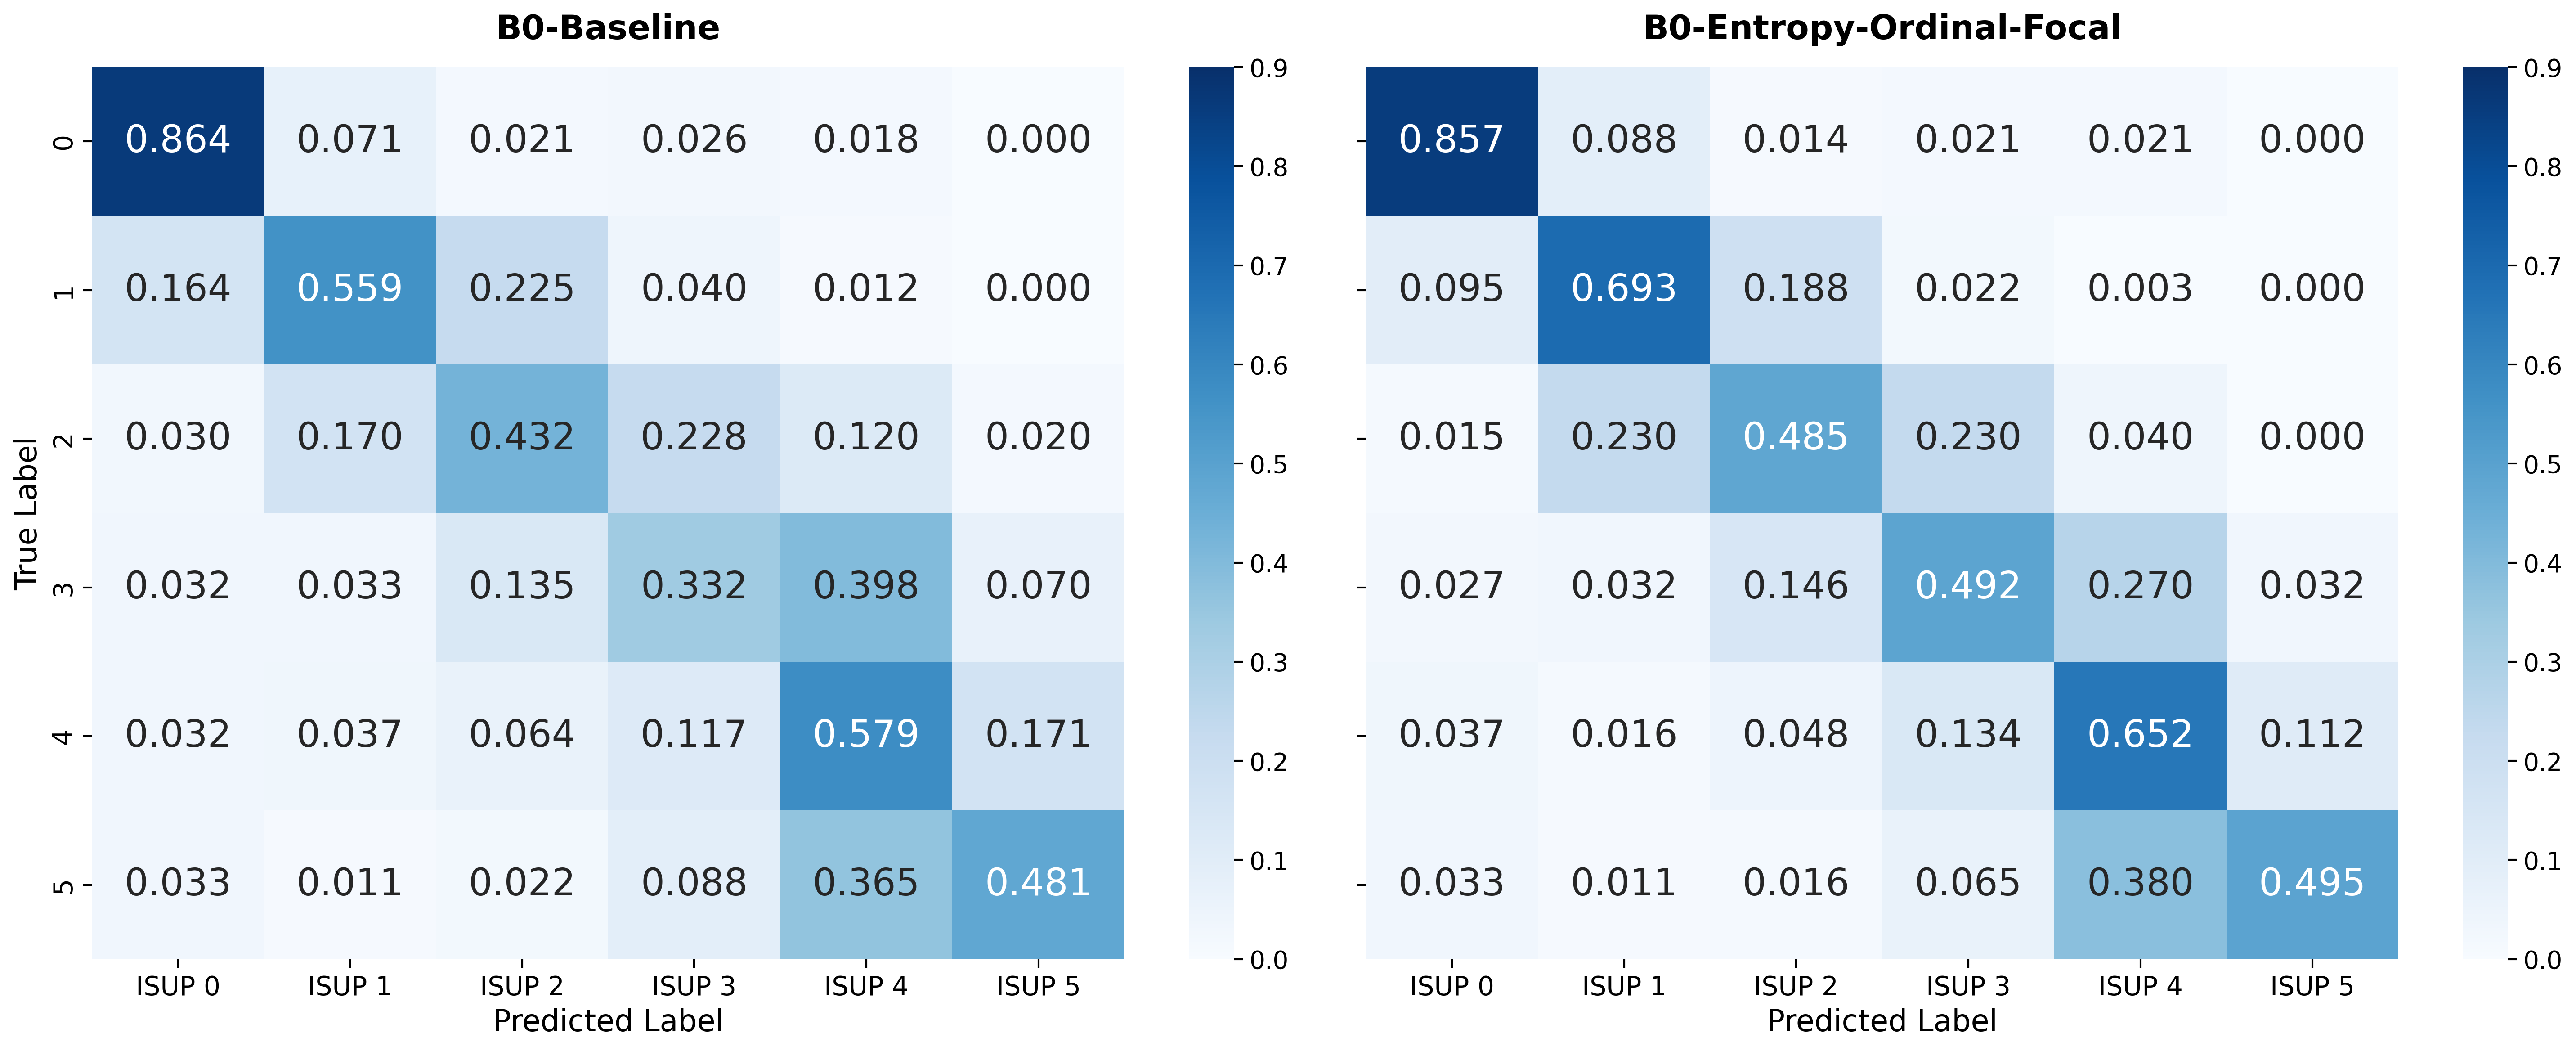
\includegraphics[width=1\linewidth]{images/comparison_cm_b0}
	\caption{Comparison between the baseline and the best individual model}
	\label{fig:comparison_b0}
\end{figure}

The analysis of the confusion matrix of the Ensemble model using the simple averaging strategy (Figure~\ref{fig:ensemble}) confirms the robustness gains observed in the global metrics, with a clear concentration of predictions along the main diagonal. The model maintains high effectiveness in identifying low-risk cases (ISUP 0 and 1) and consistent performance across the intermediate grades (ISUP 2 and 3), with errors predominantly confined to adjacent classes, in line with the expected behavior of ordinal models.
For the more aggressive grades, a complementary pattern relative to the individual models is observed. Although performance on ISUP 4 is slightly inferior to that of the B0-Entropy-Ordinal-Focal model, the Ensemble shows superior ability to identify ISUP 5 cases, reinforcing its clinical utility by prioritizing sensitivity in the histological grade associated with the worst prognosis.
\begin{figure}[H]
	\centering
	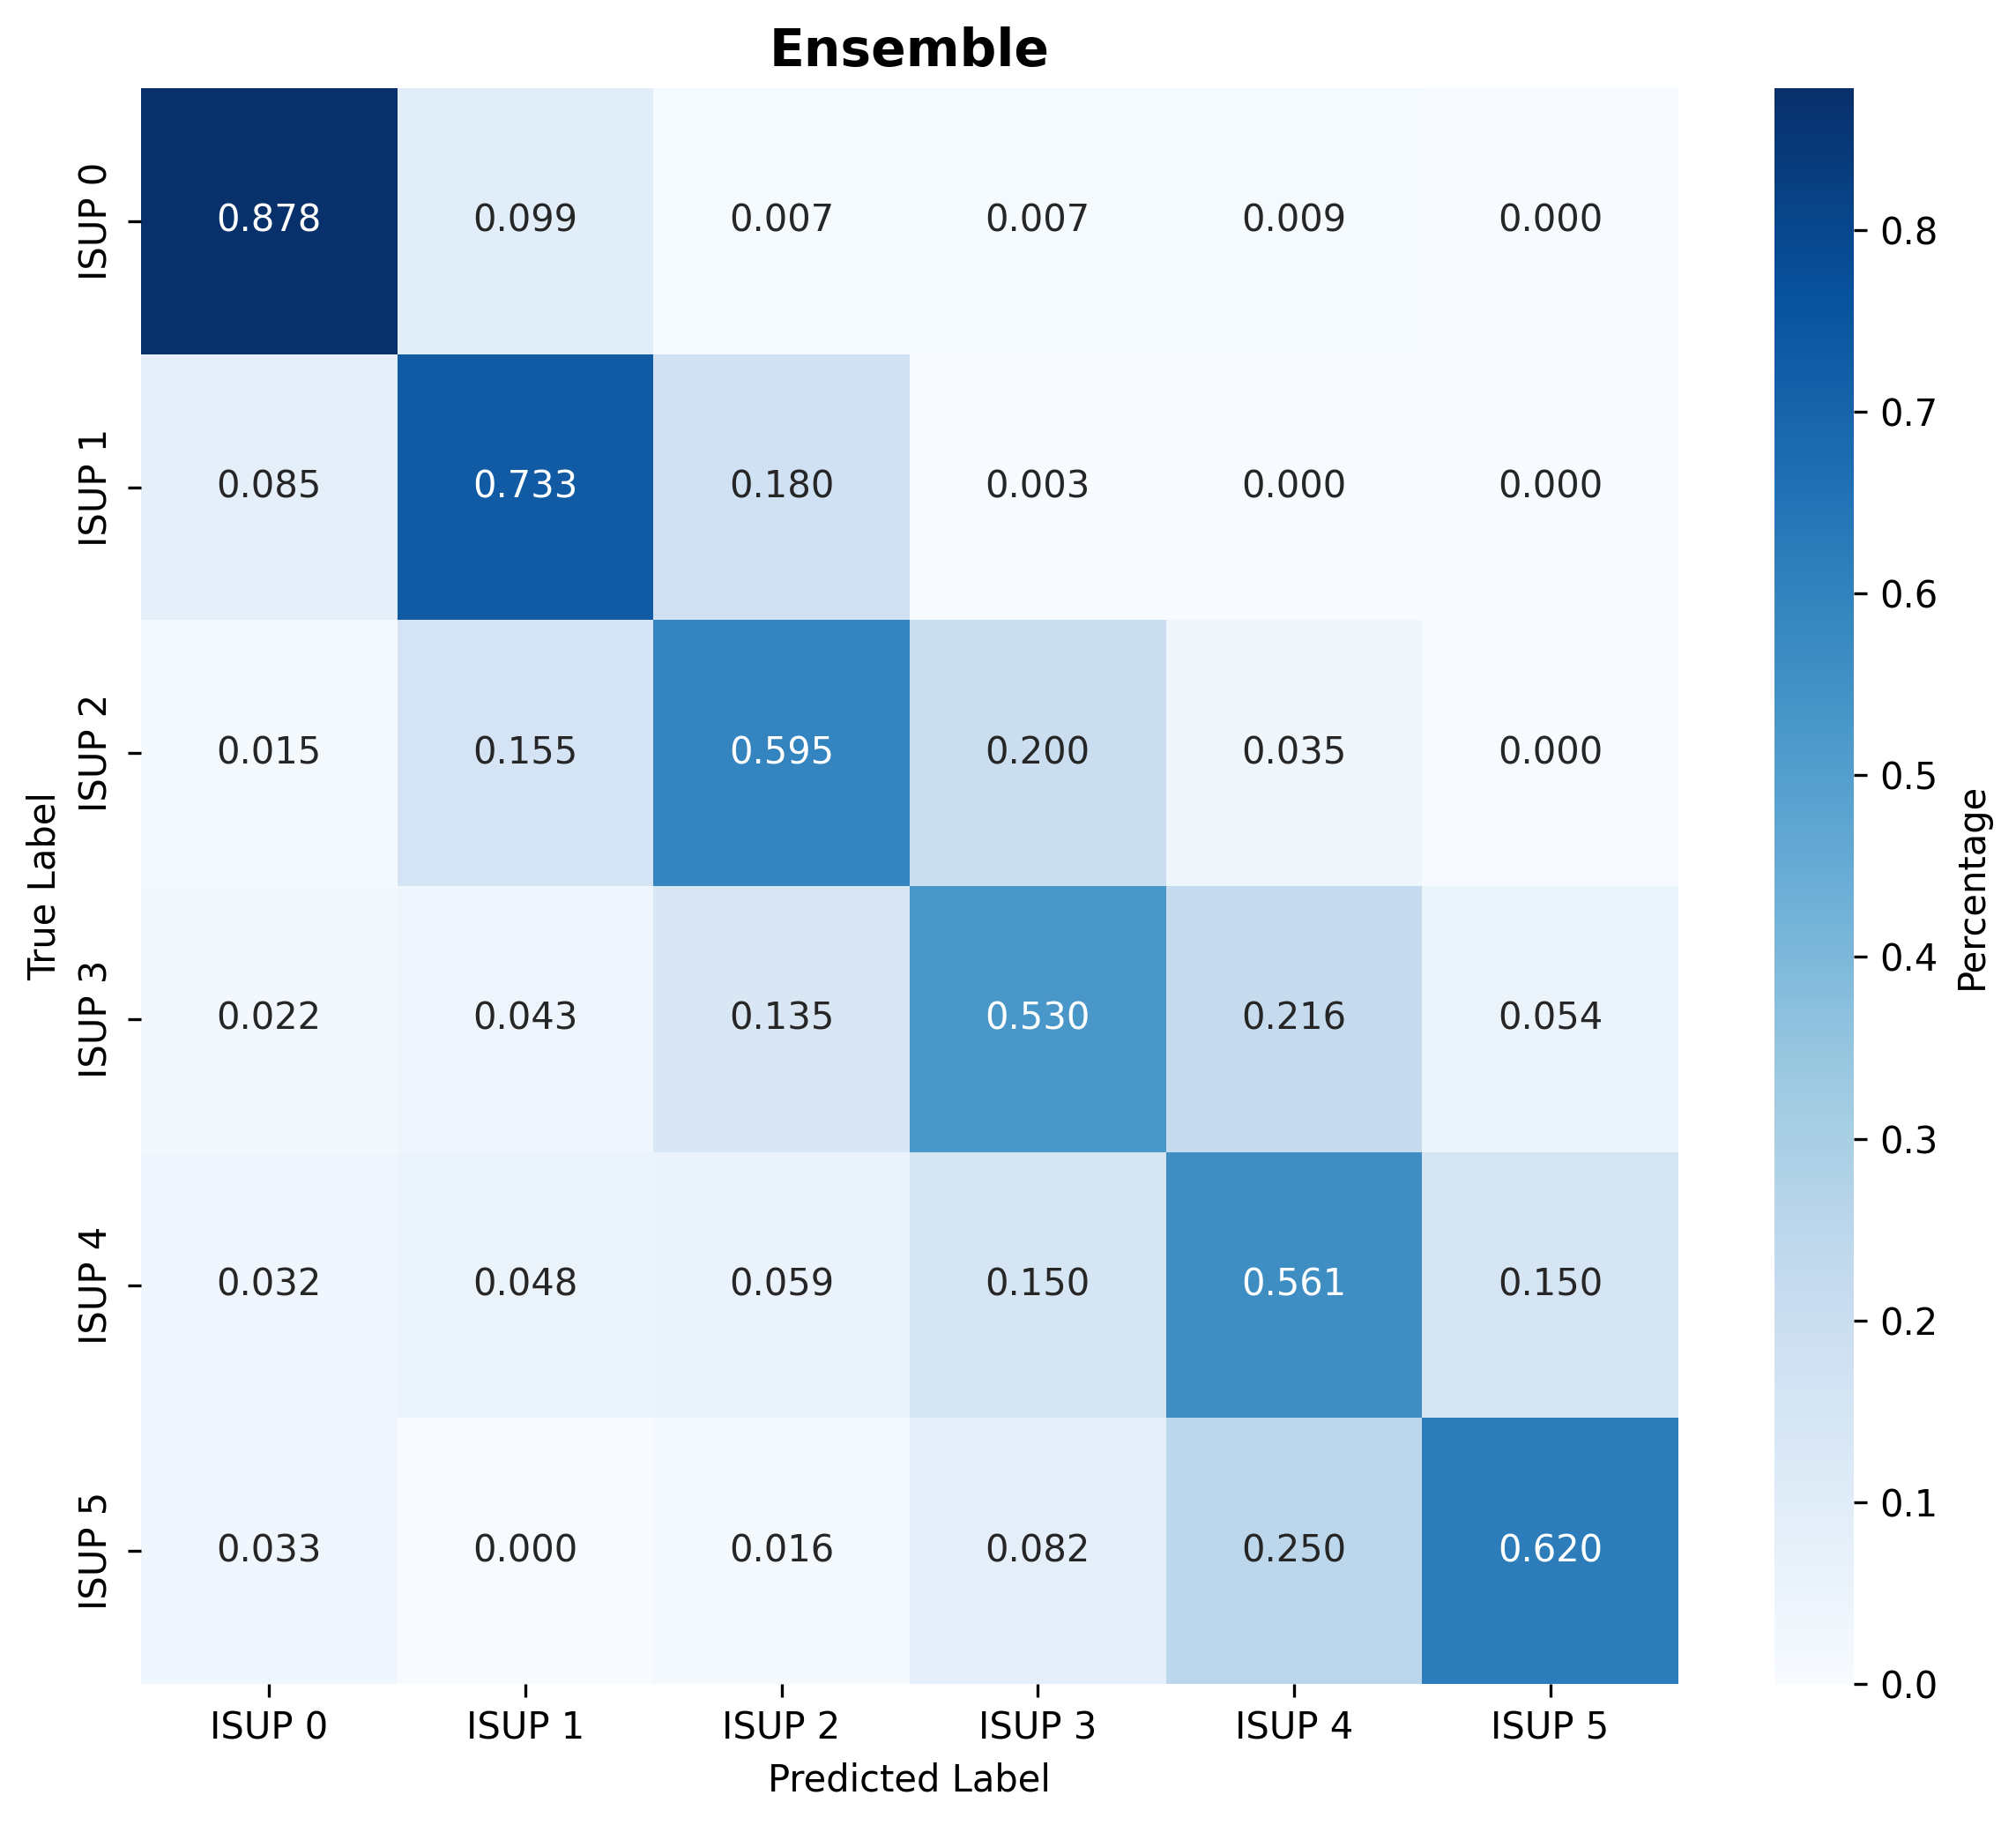
\includegraphics[width=0.8\linewidth]{images/ensemble_cm}
	\caption{Ensemble confusion matrix.}
	\label{fig:ensemble}
\end{figure}

The Table~\ref{tab:comparison-results} presents a comparison between the results obtained in this work and those reported in previous studies. Given the methodological heterogeneity in the literature, the analysis was structured around three principal axes: data complexity, performance as measured by Quadratic Weighted Kappa (QWK), and clinical consistency.

Regarding data complexity, this work uses the PANDA dataset, widely recognized for its high levels of noise and institutional variability. In contrast, studies such as those by Lucas et al. and Hammouda et al. report high performance metrics on private, smaller-scale datasets. This scenario may overestimate performance and limit the generalizability of the models.

In terms of QWK performance, the proposed model achieves competitive results, outperforming works such as those by Lucas et al. and Nagpal et al. Although Singhal et al. reported higher values, their approach relies on deeper architectures and more complex strategies, including active learning. In this study, the EfficientNet family was selected to achieve a more balanced trade-off between predictive performance and computational cost.
From a clinical perspective, although some studies report higher accuracy values, the confusion matrix analysis of the present work shows that the model more robustly preserves the ordinal structure of the problem. Most errors occur between adjacent classes, a behavior consistent with clinical practice and not adequately captured by aggregate metrics such as accuracy.


\begin{table}[H]
	\centering
	\footnotesize % Fonte menor para melhor ajuste
	\begin{tabular}{@{}lp{2.8cm}p{2cm}p{2cm}p{3cm}@{}}
		\toprule
		\textbf{Study} & \textbf{Methodology} & \textbf{Dataset} & \textbf{Performance} & \textbf{Remarks} \\
		\midrule
		
		\textbf{Proposed} & \textbf{EfficientNet Ensemble (B0-B3-B7) + Ordinal Focal} & \textbf{PANDA (10,616 WSIs)} & \textbf{QWK: 0.879, Acc: 69.8\%} & \textbf{Focus on noise reduction (Entropy) and ordinal consistency.} \\
		\midrule
		
		\cite{ref-bulten2020} & Extended U-Net & Radboud (5,759 biopsies) & QWK: 0.918 (Internal), QWK: 0.700 (External) & Outperformed 10 out of 15 pathologists. \\
		\midrule
		
		\cite{ref-singhal2022} & U-Net + ResNeXt50 & Multicenter (6,670 WSIs) & QWK: 0.93, Acc: 83.1\% & Used \textit{Active Learning} and domain adaptation. \\
		\midrule
		
		\cite{ref-nagpal2019} & InceptionV3 + k-NN & TCGA + Others (1,226 slides) & Acc: 0.70 & Significantly outperformed the average of pathologists (0.61). \\
		\midrule
		
		\cite{ref-lucas2019} & InceptionV3 & Private (96 sections) & QWK: 0.70 & Limited dataset; high accuracy only for binary classes. \\
		\midrule
		
		\cite{ref-kott2019} & ResNet-18 & Private (85 WSIs) & Acc: 85.4\% & Pilot study focused on multiclass grading. \\
		\midrule
		
		\cite{ref-hammouda2021} & Pyramidal CNN & Radboud (608 images) & Acc: 94\% & Small dataset, artificially balanced. \\
		\bottomrule
	\end{tabular}
	\caption{Comparison of the results obtained by the proposed method with related state-of-the-art works.}	
	\label{tab:comparison-results}
\end{table}